\chapter{The AlphaT Analysis}
\label{ch:5}

% **************************** Define Graphics Path **************************
\ifpdf
    \graphicspath{{Chapter5/Figs/Raster/}{Chapter5/Figs/PDF/}{Chapter5/Figs/}}
\else
    \graphicspath{{Chapter5/Figs/Vector/}{Chapter5/Figs/}}
\fi


%********************************** % First Section  *************************************
\section{Analysis Overview}  %Section - 1.1 
\label{sec:selection_analysis_overview}

In this analysis events are binned in exclusive categories of \HT, 
and the multiplicity of jets and b-tagged jets,  
\nj and \nb. Such binning allows for targeted interpretations across
the vast array of
possible simplified model final states, while reducing background yields to a 
minimum.

Analyses searching in the jets and \met final state encounter significant 
backgrounds from SM sources of both genuine \met [with associated jet production] 
and fake \met, originating from jet mis-measurement. The \alphat 
analysis makes predictions for the former using a data-driven transfer factor 
technique to extrapolate yields from statistically independent control samples 
into the signal region. However the latter, sources of fake \met from QCD multijet events,
are reduced to a negligible level using the kinematic 
variable \alphat.

The main analysis signal region is described in the remainder of this chapter,
with background prediction techniques detailed later in chapter~\ref{ch:6}.


\subsection{The \alphat kinematic variable}
\label{sec:alphat}

QCD multijet (MJ) events dominate the SM background in any search with multiple jets 
in the final state. Jet mis-measurements in a 
purely QCD MJ event can lead to non-negligible amounts of \mht, therefore 
passing the signal selection. Attempting
to accurately measure this contribution is
made very difficult given the hadronic environment of the LHC, and the lack of 
precise measurements and calculations of the large multijet cross sections. As an 
alternative approach, the goal of this analysis is to reduce QCD down to an
entirely negligible level. This is 
achieved with the dimensionless kinematic variable, \alphat [REF]. This is defined
for dijets as:

\begin{equation}
\alphat = \frac{E_T^{j_2}}{M_T}
\label{eq:alphat_dijet}
\end{equation}

where $E_T^{j_2}$ is the transverse energy of the less energetic jet and $M_T$ 
is the transverse mass of the dijet system, defined as:

\begin{equation}
M_T = \sqrt{\bigg(\sum^2_{i=1}{E_T^{j_i}}\bigg)^2 - \bigg(\sum^2_{i=1}{p_x^{j_i}}\bigg)^2 - \bigg(\sum^2_{i=1}{p_y^{j_i}}\bigg)^2}
\label{eq:mt}
\end{equation}

where $E_T^{j_i}$, $p_x^{j_i}$ and $p_y^{j_i}$ are the transverse energy and 
transverse momentum in the $x$ and $y$ planes, for the jet $j_i$.

The \alphat variable can be generalised to an n-jet case by considering the event as a 
pseudo-dijet system, constructing each pseudo-jet such that the difference in \HT
between each pseudo-jet system, \deltaHT, is minimised. \alphat then takes the 
form:

\begin{equation}
\alphat = \frac{1}{2} \times \frac{\HT-\deltaHT}{\sqrt{\HT^2 - \mht^2}} = 
\frac{1}{2} \times \frac{1-\frac{\deltaHT}{\HT}}{\sqrt{1 - \frac{\mht}{\HT}^2}}
\label{eq:alphat_njet}
\end{equation}

A perfectly measured dijet event containing back to back jets in $\phi$ of equal energy will
have an \alphat value of 0.5, whereas 
events with \mht originating from jet energy mismeasurements will have values of $\alphat<0.5$.
Events containing sources of genuine \met, whether from SM or BSM sources, can have values
of $\alphat > 0.5$.

\emph{show plots of correlations between \mht and \deltaHT for QCD, 
signal, SM real MET etc.}


%********************************** % First Section  *************************************
\section{Hadronic Signal Region}
\label{sec:selection_hadronic}
% Introduce that QCD is a dominant background due to jet mis-measurement.

This section outlines the relevant background sources of this analysis, and
describes the basic hadronic pre-selection made for the signal 
region, as well as the relevant trigger requirements and data and 
simulation samples used.

\subsection{SM Backgrounds}
SM backgrounds are categorized into sources of genuine and fake 
missing energy.

\subsubsection{Genuine EWK \met}
Events containing leptonic decays of W bosons, \wlnu, originating either
from direct W prodution, or via the decay of a top quark, are sources of genuine 
missing energy. The presence of a weakly interacting neutrino which evades
detection leads to an energy imbalance. Such events are vetoed in the signal
region due to the presence of a 
lepton, however if the lepton is missed for whatever reason, leptonic W decays 
can pass the signal selection, forming a significant SM background.

% While lepton and photon vetoes employed in the signal region surpress 
% significant amounts of background from events with neutrinos, such events can 
% still persist if, for example, the lepton is not identified.
% Such processes are predominantly from \ttbar or W-boson production, where the 
% W decays via \wlnu. If the lepton is `lost' and evades our 
% lepton vetoes, significant missing energy can be produced not only from missing 
% the lepton, but from the presence of the neutrino. When such processes are accompanied 
% by associated jet production they are then able to pass our signal region selection.

Leptons can be `lost' for a variety different reasons, but ultimately for failing
the lepton ID criteria. There are numerous potential causes, the 
most prevelant being soft-leptons below ID threshold or non-isolated leptons 
which pass the ID quality cuts but fail the isolation requirement.

\emph{SHOW TABLE WITH THE BACKGROUND BREAKDOWN - PUT INTO GRAPHICAL FORM?}

Events containing a Single Isolated Track (SIT) are vetoed from the signal 
region. While originally designed to target hadronically decaying tau leptons, 
this requirement reduces the remaining lost-lepton backgrounds also.

The dominant EWK source of genuine missing energy comes from a Z-boson 
production where the Z decays
via neutrinos, \zinv, with associated jet production. This source of background
is considered irreducible.

Following the reduction of such processes using the lepton, photon and SIT vetoes,
any remaining contributions from SM EWK backgrounds are estimated using a 
fully data-driven transfer factor technique, described in detail in
Section~\ref{sec:background_overview}.

\subsubsection{Fake MET}

As mentioned previously, the dominant source of background for analyses 
searching for a multijet final state is from QCD. A fully-measured QCD event 
would consist of multiple jets balancing each other in all planes, however in 
order to enter the signal region, an event must contain missing energy, 
\mht (equivalent to \met in all-hadronic events).

The most common way for a balanced multijet (MJ) event to gain \mht is when one 
or more of the jets are mis-measured, such that their vectorial sum then leads to non-zero
\mht. This can due to badly calibrated or damaged segments of the calorimeter 
systems, or due to stochastic fluctuations within the jet-resolution of the 
detector. The former is protected against using a `dead ECAL filter', where 
events are vetoed if they contain significant energy deposits within a given 
distance from areas of the calorimeter system known to be either dead or 
damaged. The latter is dealt with using a cut on the \alphat variable where 
events with fake missing energy signatures give values $<0.5$.

QCD MJ events can also appear to contain non-zero missing energy 
due to the threshold requirements of jets. If an event contains 
one or more jets below the analysis threshold, then the 
event becomes imbalanced and will contain \mht. Events such as these are largely 
removed with the \alphat requirement, however in addition a requirement is made on the
ratio \mhtmet.

\subsection{Selection Criteria}
\label{sec:selec_crit}
The hadronic signal region
requires at least 2 jets and that the topology has a value of \alphat greater than
0.55. While no absolute \met requirement is made, the cut on 
\alphat imposes an implied threshold, which maintains the analysis'
sensitivity to very low regions of \met. Events are also required to have at least
$\HT > 200$\gev ensuring the presence of significant hadronic activity.

Any events containing leptons or photons are vetoed to ensure purely hadronic events
are considered, thereby surpressing events with genuine \met from leptonic decays to
neutrinos.

It is possible for events to acquire significant amounts of \mht without having any
real \met present when multiple jets are below the analysis threshold. To protect against 
this scenario, events are required to have a low ratio of the two variables, specifically
\mhtmet < 1.25.

Events can also acquire fake \mht if they overlap with areas of the calorimater 
system which are damaged or known to be faulty, where jets can be mis-measured or 
lost as a result. To protect against this, for a given jet $j$, the angular seperation
between the event \mht, calculated excluding jet $j$, and the jet itself is used, defined
as:

\begin{equation}
\Delta \phi^*_j = \Delta \phi\big(\overrightarrow{\Pt}_j,-\sum_{i\neq j}{\overrightarrow{\Pt}_i}\big)
\label{eq:biasdphi}
\end{equation}

A small value of $\Delta \phi^*_j$ indicates that the momentum vector of $j$
is aligned with the \mht vector, implying the jet is mis-measured. Events are 
vetoed if a jet with $\Delta \phi^*<0.5$ is within $\Delta R < 0.3$ of a known
`dead' region of the ECAL.

Following this preselection, events are further categorized into the three 
binning dimenions of \HT, \nb and \nj, as shown in table~\ref{tab:ht-bins}. Two 
jet multiplicity categories are defined as 2 or 3 jets, and 4 or more. B-tagged 
jet multiplicities are exactly 0, 1, 2, 3 or 4 and more. Combinations of these 
various categories are then further sub-divided into multiple \HT bins ranging 
from 200\gev up to an inclusive bin of $\HT>1075$\gev.

\begin{table}[ht!]
  \caption{\HT binning used for each \nj and \nb category.\label{tab:ht-bins}}
  \centering
  % \scriptsize % too big to fit on page
  \tiny
  \begin{tabular}{ lrrrrrrrrrrr }
    \hline
    \hline
    (\nj,\nb)       & \multicolumn{11}{c}{\HT bins (\gev)}                                                                                \\
    \hline
    (2-3,0)           & 200--275 & 275--325 & 325--375 & 375--475 & 475--575 & 575--675 & 675--775 & 775--875 & 875--975 & 975--1075 & $>$1075  \\
    (2-3,1)           & 200--275 & 275--325 & 325--375 & 375--475 & 475--575 & 575--675 & 675--775 & 775--875 & 875--975 & 975--1075 & $>$1075  \\
    (2-3,2)           & 200--275 & 275--325 & 325--375 & 375--475 & 475--575 & 575--675 & 675--775 & 775--875 & $>$875   & \multicolumn{2}{c}{} \\
%    (2-3,3)          & 200--275 & 275--325 & 325--375 & 375--475 & 475--575 & 575--675 & 675--775 & 775--875 & $>$875   & \multicolumn{2}{c}{} \\
    ($\geq$4,0)       & 200--275 & 275--325 & 325--375 & 375--475 & 475--575 & 575--675 & 675--775 & 775--875 & 875--975 & 975--1075 & $>$1075  \\
    ($\geq$4,1)       & 200--275 & 275--325 & 325--375 & 375--475 & 475--575 & 575--675 & 675--775 & 775--875 & 875--975 & 975--1075 & $>$1075  \\
    ($\geq$4,2)       & 200--275 & 275--325 & 325--375 & 375--475 & 475--575 & 575--675 & 675--775 & 775--875 & $>$875   & \multicolumn{2}{c}{} \\
    ($\geq$4,3)       & 200--275 & 275--325 & 325--375 & 375--475 & 475--575 & 575--675 & 675--775 & 775--875 & $>$875   & \multicolumn{2}{c}{} \\
    ($\geq$4,$\geq$4) & 200--275 & 275--325 & 325--375 & $>$375   & \multicolumn{7}{c}{}                                                        \\
    \hline
    \hline
  \end{tabular}
\end{table}

For bins of $\HT>375$\gev the leading two jets in the event are required to 
have $\Pt>100$\gev, with all additional jets having half the requirement of
$\Pt>50\gev$. In order to maintain a similar kinematic phase space throughout
the many \HT bins, these jet \Pt requirements are scaled for the lower \HT bins 
as shown in Table~\ref{tab:jet_pt_thresholds}.

\begin{table}[ht!]
  \caption{Jet \Et thresholds per \HT bin.\label{tab:jet_pt_thresholds}}
  \centering
  \footnotesize
  \begin{tabular}{ lcccc }
    \hline
    \hline
    \HT bin    & 200--275 & 275--325 & 325--375 & $>$375 \\
    \hline
    Lead jet       & 73.3     & 73.3     & 86.7     & 100.0  \\
    Second jet     & 73.3     & 73.3     & 86.7     & 100.0  \\
    All other jets & 36.7     & 36.7     & 43.3     & 50.0   \\
    \hline
    \hline
  \end{tabular}
\end{table}

Example distributions of \alphat, \HT, \mht and jet \Pt  are shown in
figure~\ref{fig:datamc_had_inc}, comparing data against MC.

\begin{figure}[!ht]
  \centering
    \begin{subfigure}[b]{0.48\textwidth}
      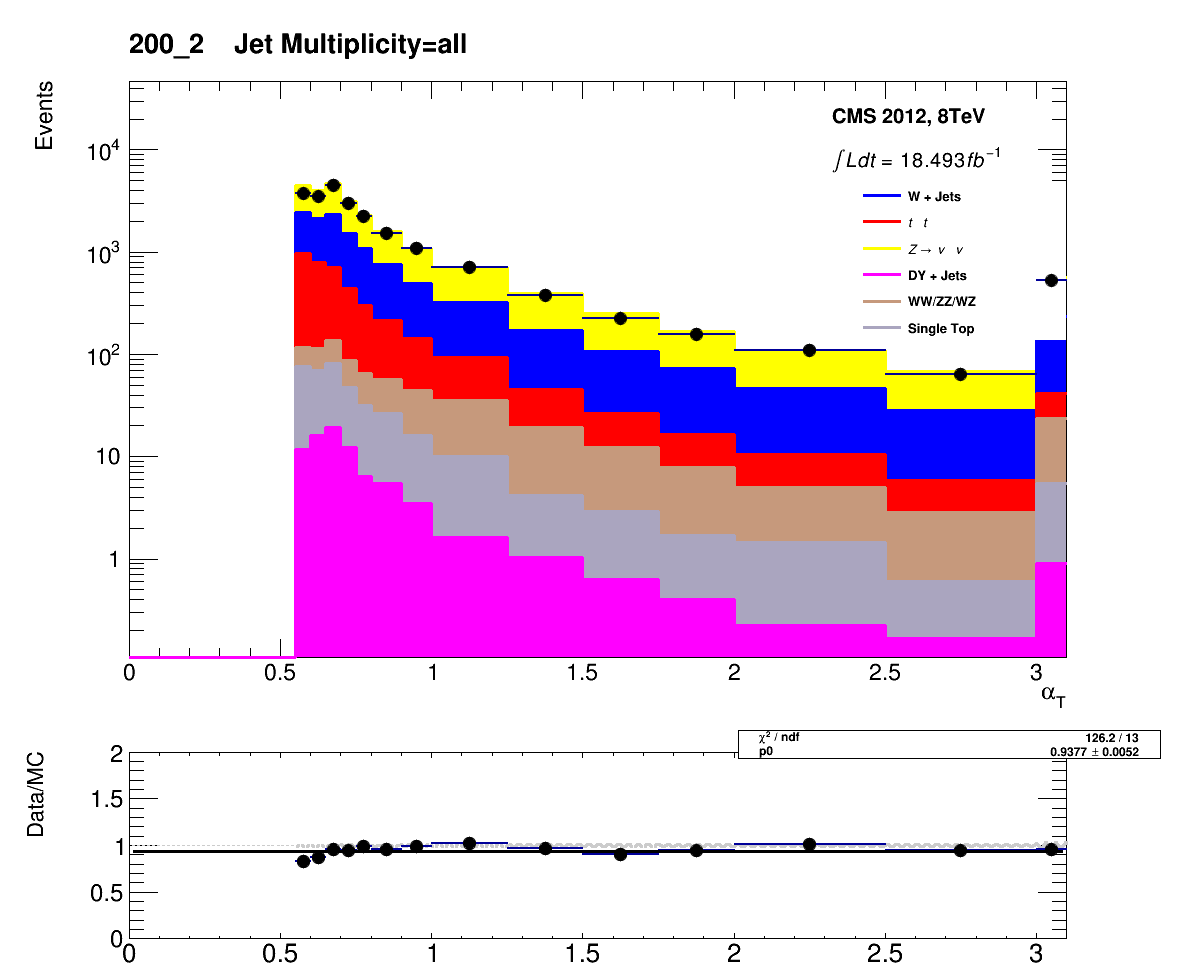
\includegraphics[width=\textwidth]{Figs/datamc/had/Stacked_AlphaT_all_200_upwards}
      \caption{\alphat}
    \end{subfigure}
    \begin{subfigure}[b]{0.48\textwidth}
      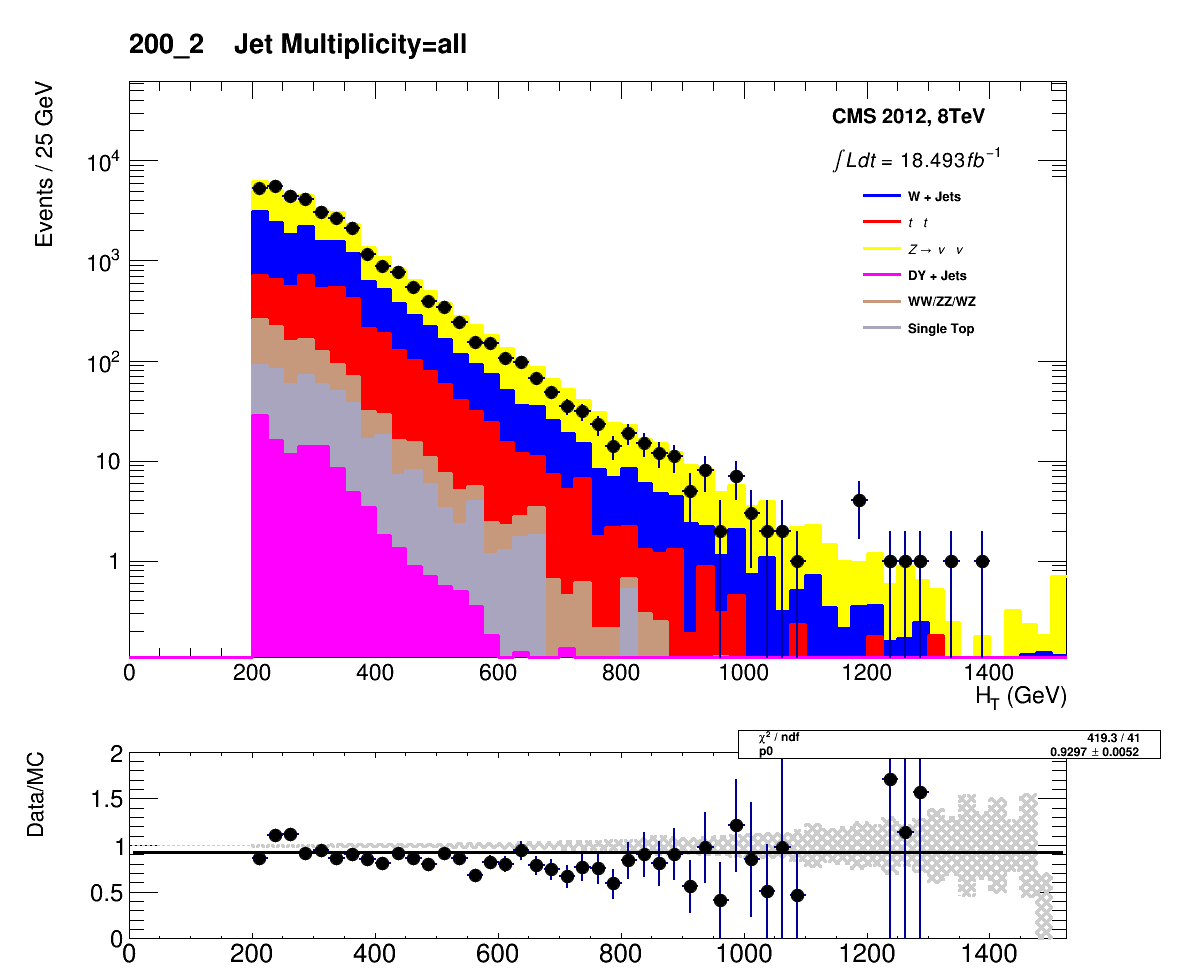
\includegraphics[width=\textwidth]{Figs/datamc/had/Stacked_HT_all_200_upwards}
      \caption{\HT}
    \end{subfigure} \\
    \begin{subfigure}[b]{0.48\textwidth}
      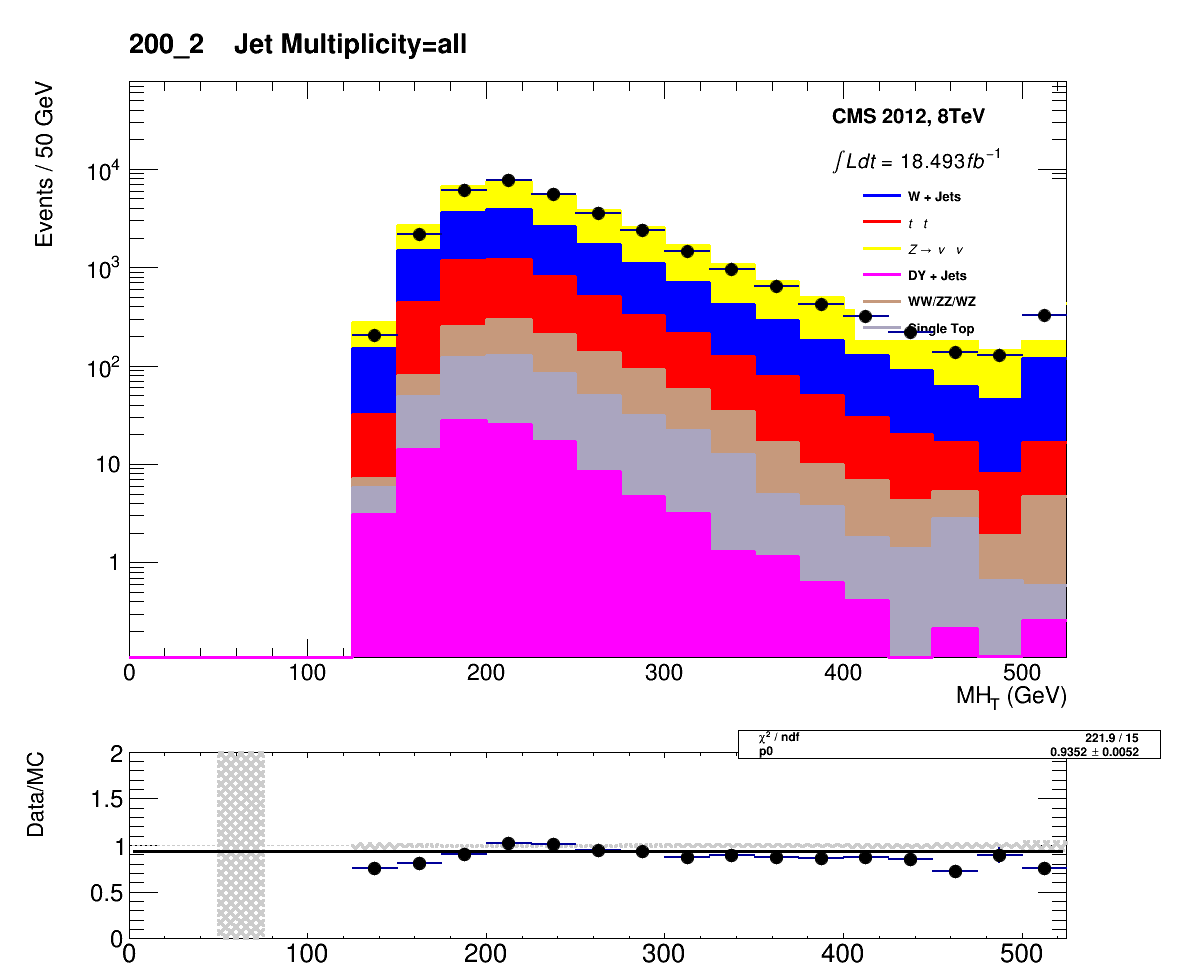
\includegraphics[width=\textwidth]{Figs/datamc/had/Stacked_MHT_all_200_upwards}
      \caption{\mht}
    \end{subfigure}
    \begin{subfigure}[b]{0.48\textwidth}
      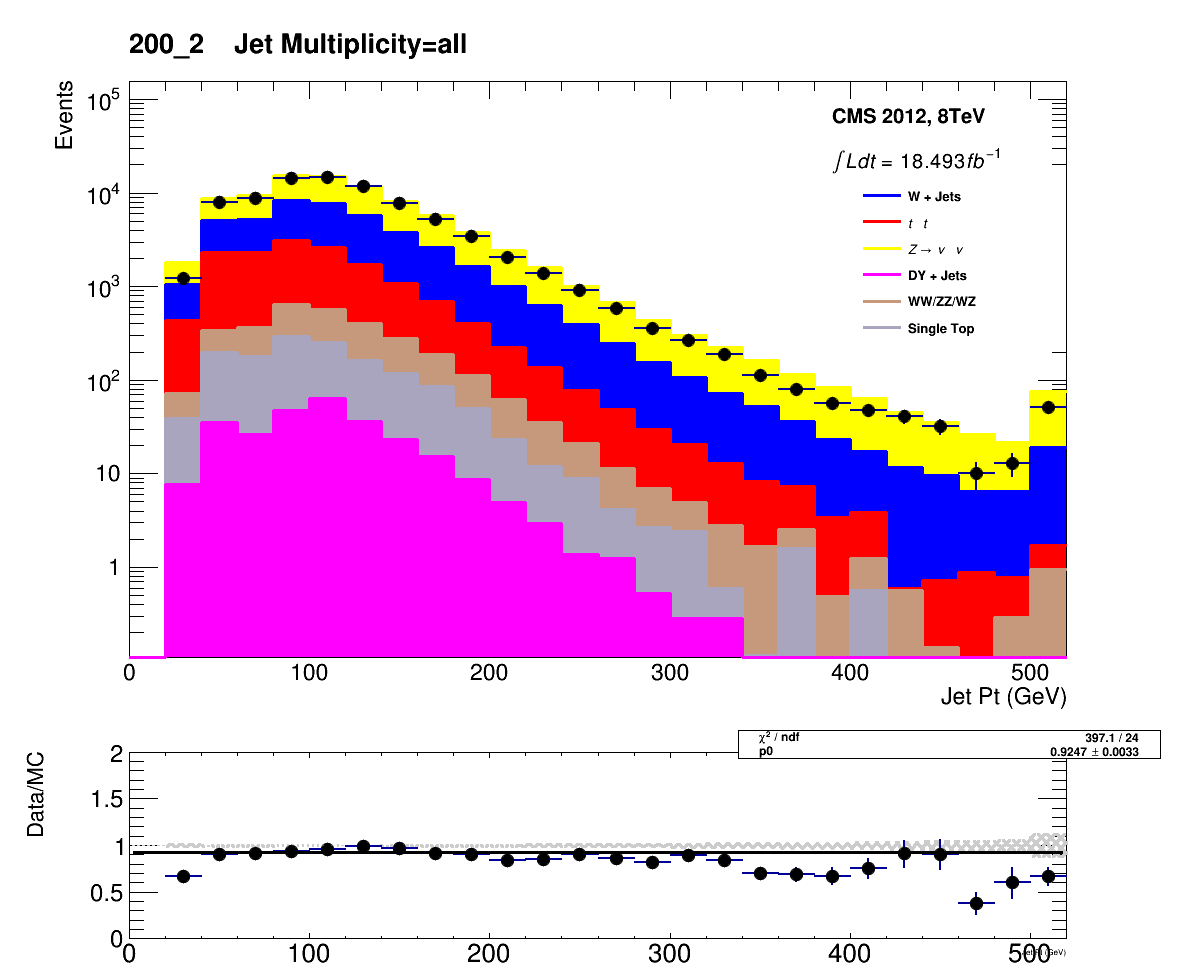
\includegraphics[width=\textwidth]{Figs/datamc/had/Stacked_CommonJetPt_all_200_upwards}
      \caption{Jet \Pt}
    \end{subfigure} \\
    \caption{\label{fig:datamc_had_inc}
    Comparison of data with MC for the full hadronic signal selection. Plots 
    are for $\HT>200\gev, \nj\geq2, \nb\geq0$.
    }
\end{figure}

\subsection{Signal Triggers}

\emph{Add emphasis on parked trigger, as it opens up phase space to compressed susy models}

Events are collected at the HLT using a dedicated suite of
signal triggers. For an event to pass the trigger
requirements, it must exceed both a \HT and an \alphat threshold. Trigger rate 
can be maintained by varying the
threshold requirement on each of these independent `legs', as shown in Table~
\ref{tab:sig_trigs}. Each \HT bin in the analysis is seeded by a single trigger,
with a 25\gev offset in online and offline \HT, with the exception of the 200
\gev bin.

% \begin{table}[h]
% \begin{tabular}{l|l}
% HT bin (\gev) & HLT Trigger            \\ \hline
% 200-275       & HLT\_HT200\_AlphaT0p57 \\
% 275-325       & HLT\_HT200\_AlphaT0p57 \\
% 325-375       & HLT\_HT300\_AlphaT0p53 \\
% 375-475       & HLT\_HT350\_AlphaT0p52 \\
% 475-575       & HLT\_HT400\_AlphaT0p51 \\
% 575-675       & HLT\_HT400\_AlphaT0p51 \\
% 675-775       & HLT\_HT400\_AlphaT0p51 \\
% 775-875       & HLT\_HT400\_AlphaT0p51 \\
% 875-975       & HLT\_HT400\_AlphaT0p51 \\
% 975-1075      & HLT\_HT400\_AlphaT0p51 \\
% 1075-$\inf$   & HLT\_HT400\_AlphaT0p51 \\
% \end{tabular}
% \label{tab:sig_trigs}
% \end{table}

\begin{table}[!ht]
  \caption{Signal triggers, the L1 seed triggers and their efficiencies measured
  for per \HT and \nj category.}
  \label{tab:sig_trigs}
  \centering
  \scriptsize
  \begin{tabular}{ cccccc }
    \hline
    \hline
    Offline \HT       & Offline \alphat & L1 seed (\verb!L1_?!)         & Trigger (\verb!HLT_?!)  & \multicolumn{2}{c}{Efficiency (\%)}          \\ [0.5ex]
    region (\gev)         & threshold       & (highest thresholds)          &                         & $2 \leq \nj \leq 3$ & $\nj \geq 4$       \\ [0.5ex]
    \hline
    $200 < \HT < 275$ & 0.65            & \verb!DoubleJetC64!           & \verb!HT200_AlphaT0p57! & $81.8^{+0.4}_{-0.4}$  & $78.9^{+0.3}_{-0.4}$ \\
    $275 < \HT < 325$ & 0.60            & \verb!DoubleJetC64!           & \verb!HT200_AlphaT0p57! & $95.2^{+0.3}_{-0.4}$  & $90.0^{+1.2}_{-1.3}$ \\
    $325 < \HT < 375$ & 0.55            & \verb!DoubleJetC64 OR HTT175! & \verb!HT300_AlphaT0p53! & $97.9^{+0.3}_{-0.3}$  & $95.6^{+0.9}_{-1.0}$ \\
    $375 < \HT < 475$ & 0.55            & \verb!DoubleJetC64 OR HTT175! & \verb!HT350_AlphaT0p52! & $99.2^{+0.2}_{-0.2}$  & $98.7^{+0.5}_{-0.7}$ \\
    $\HT > 475$       & 0.55            & \verb!DoubleJetC64 OR HTT175! & \verb!HT400_AlphaT0p51! & $99.8^{+0.1}_{-0.3}$  & $99.6^{+0.3}_{-0.7}$ \\
    \hline
    \hline
  \end{tabular}
\end{table}

Trigger efficiencies are measured against an unbiased muon reference trigger,
\\\verb!HLT_IsoMu24_eta2p1!, using a muon tag and probe method where a
single muon is selected and then subsequently ignored from the analysis when 
calculating event level variables such as \HT, \mht and \alphat. Efficiencies 
are measured for each \HT bin and for each \nj category, as summarised in 
table~\ref{tab:sig_trigs}. Example trigger turn on curves are shown for the 3 
lowest \HT bins in figures~\ref{fig:eff_alphat_le3j} and \ref{fig:eff_alphat_ge4j}.
Across the higher \HT 
bins the triggers are fully efficient, with some inefficiencies seen only in the
lower \HT bins. These innefficiencies are understood as being due to the L1 seed
trigger used for this region, which had high thresholds in order to maintain 
low rates in the high PU environment throughout \runone. Lower 
efficiencies are also observed in the \njhigh category attributed to the presence of 
softer jets, as an increased number of jets must equate to the same total \HT 
requirement of the bin.

\begin{figure}[!ht]
  \centering
    
    \begin{subfigure}[b]{0.48\textwidth}
      
\includegraphics[width=\textwidth,page=11]{figures/trigger/HT200_275_73_73_36_AlphaT_le3j_RunAtFNAL}
      \caption{Differential, $200 < \HT < 275 $\gev}
    \end{subfigure}
    \begin{subfigure}[b]{0.48\textwidth}
      
\includegraphics[width=\textwidth,page=18]{figures/trigger/HT200_275_73_73_36_AlphaT_le3j_RunAtFNAL}
      \caption{Cumulative, $200 < \HT < 275 $\gev}
    \end{subfigure} \\
    \begin{subfigure}[b]{0.48\textwidth}
      
\includegraphics[width=\textwidth,page=11]{figures/trigger/HT275_325_73_73_36_AlphaT_le3j_RunAtFNAL}
      \caption{Differential, $275 < \HT < 325 $\gev}
    \end{subfigure}
    \begin{subfigure}[b]{0.48\textwidth}
      
\includegraphics[width=\textwidth,page=18]{figures/trigger/HT275_325_73_73_36_AlphaT_le3j_RunAtFNAL}
      \caption{Cumulative, $275 < \HT < 325 $\gev}
    \end{subfigure} \\
    \begin{subfigure}[b]{0.48\textwidth}
      
\includegraphics[width=\textwidth,page=11]{figures/trigger/HT325_375_86_86_43_AlphaT_le3j_RunAtFNAL}
      \caption{Differential, $325 < \HT < 375 $\gev}
    \end{subfigure}
    \begin{subfigure}[b]{0.48\textwidth}
      
\includegraphics[width=\textwidth,page=18]{figures/trigger/HT325_375_86_86_43_AlphaT_le3j_RunAtFNAL}
      \caption{Cumulative, $325 < \HT < 375 $\gev}
    \end{subfigure} \\
  
    \caption{\label{fig:eff_alphat_le3j}
      \emph{Maybe drop the differential turn-ons and just keep the cumu.}
      Differential (left) and Cumulative (right) efficiency turn-on curves for 
      the signal triggers, for the three lowest \HT bins and \njlow.}
\end{figure}

\begin{figure}[!ht]
  \centering
    
    \begin{subfigure}[b]{0.48\textwidth}
      
\includegraphics[width=\textwidth,page=11]{figures/trigger/HT200_275_73_73_36_AlphaT_ge4j_RunAtFNAL}
      \caption{Differential, $200 < \HT < 275 $\gev}
    \end{subfigure}
    \begin{subfigure}[b]{0.48\textwidth}
      
\includegraphics[width=\textwidth,page=18]{figures/trigger/HT200_275_73_73_36_AlphaT_ge4j_RunAtFNAL}
      \caption{Cumulative, $200 < \HT < 275 $\gev}
    \end{subfigure} \\
    \begin{subfigure}[b]{0.48\textwidth}
      
\includegraphics[width=\textwidth,page=11]{figures/trigger/HT275_325_73_73_36_AlphaT_ge4j_RunAtFNAL}
      \caption{Differential, $275 < \HT < 325 $\gev}
    \end{subfigure}
    \begin{subfigure}[b]{0.48\textwidth}
      
\includegraphics[width=\textwidth,page=18]{figures/trigger/HT275_325_73_73_36_AlphaT_ge4j_RunAtFNAL}
      \caption{Cumulative, $275 < \HT < 325 $\gev}
    \end{subfigure} \\
    \begin{subfigure}[b]{0.48\textwidth}
      
\includegraphics[width=\textwidth,page=11]{figures/trigger/HT325_375_86_86_43_AlphaT_ge4j_RunAtFNAL}
      \caption{Differential, $325 < \HT < 375 $\gev}
    \end{subfigure}
    \begin{subfigure}[b]{0.48\textwidth}
      
\includegraphics[width=\textwidth,page=18]{figures/trigger/HT325_375_86_86_43_AlphaT_ge4j_RunAtFNAL}
      \caption{Cumulative, $325 < \HT < 375 $\gev}
    \end{subfigure} \\
  
    \caption{\label{fig:eff_alphat_ge4j}
      \emph{Maybe drop the differential turn-ons and just keep the cumu.}
      Differential (left) and Cumulative (right) efficiency turn-on curves for 
      the signal triggers, for the three lowest \HT bins and \njhigh.}
\end{figure}

All triggers were present throughout \runone, however the 
\\\verb!HLT_HT200_AlphaT0p57! trigger was used as part of the `Parked' stream of 
data which was reconstructed at a later date, following the active data-taking 
period. During data taking triggers may have `prescale' factors applied to them 
such that only every $n$ triggered events are actually recorded, however all of
the signal triggers remained unprescaled for the entirety of the 8\tev
data-taking.



\subsection{Formula method}

tie in with the split into nb and nj categories - necessary as stats will reduce, so we use
this `trick' to reduce errors



\section{Datasets and MonteCarlo samples}

\subsection{Datasets}

The datasets used in this analysis are listed in Table~\ref{tab:datasets}. These
include the primary signal sample datasets, named `HTMHTParked', for which only
Run2012A is absent as the parked trigger was present only during the 
run period's B, C and D. All other datasets contain events from triggers used for 
background estimation.

\begin{table}[ht]
  \caption{8\tev Datasets.}
  \label{tab:datasets}
  \centering
  \scriptsize
  \begin{tabular}{ lc }
    \hline
    \hline
    Dataset & Luminosity (fb$^{-1}$) \\
    \hline
    \verb!/HTMHTParked/Run2012B-22Jan2013-v1/AOD! & 4.41 \\
    \verb!/HTMHTParked/Run2012C-22Jan2013-v1/AOD! & 6.80 \\
    \verb!/HTMHTParked/Run2012D-22Jan2013-v1/AOD! & 7.29 \\
    \multicolumn{1}{r}{Total} & 18.49 \\ [0.5ex]
    \verb!/HT/Run2012A-22Jan2013-v1/AOD! & n/a \\
    \verb!/JetHT/Run2012B-22Jan2013-v1/AOD! & n/a \\
    \verb!/JetHT/Run2012C-22Jan2013-v1/AOD! & n/a \\
    \verb!/JetHT/Run2012D-22Jan2013-v1/AOD! & n/a \\
    \multicolumn{1}{r}{Total} & 18.33 \\ [0.5ex]
    \verb!/SingleMu/Run2012A-22Jan2013-v1/AOD! & 0.69 \\
    \verb!/SingleMu/Run2012B-22Jan2013-v1/AOD! & 4.40 \\
    \verb!/SingleMu/Run2012C-22Jan2013-v1/AOD! & 6.77 \\
    \verb!/SingleMu/Run2012D-22Jan2013-v1/AOD! & 7.27 \\
    \multicolumn{1}{r}{Total} & 19.13 \\ [0.5ex] % 19.13
    \verb!/Photon/Run2012A-22Jan2013-v1/AOD! & 0.68 \\
    \verb!/SinglePhoton/Run2012B-22Jan2013-v1/AOD! & 4.40 \\
    \verb!/SinglePhoton/Run2012C-22Jan2013-v1/AOD! & 6.77 \\
    \verb!/SinglePhotonParked/Run2012D-22Jan2013-v1/AOD! & 7.27 \\
    \multicolumn{1}{r}{Total} & 19.12 \\ [0.5ex] % 19.18
    \hline
    \hline
  \end{tabular}
\end{table}

\subsection{MonteCarlo Background and Signal samples}

The full list of MonteCarlo (MC) samples used in this analysis are listed in 
Table~\ref{tab:mc-sm} along with the number of events, next-to-next-to-leading 
order (NNLO) cross section and an effective integrated luminosity for each.

\emph{can describe the different methods of MC generation}

Each sample is weighted such that it's effective integrated luminosity is 
made equivalent to the relevant dataset luminosity. Event-by-event weights are applied 
such that the sample's PU distribution matches that as measured in data.

\begin{landscape}
  \begin{center}
    \begin{table}[ht]
      \caption{MC samples for Standard Model processes.}
      \label{tab:mc-sm}
      \centering
      \tiny
      \begin{tabular}{ lrrrr }
        \hline
        Sample & N$_{\textrm{event}}$ & Cross section (pb) & Corrected Cross section (pb) & Luminosity (fb$^{-1}$) \\
        \hline
        \hline
        \verb!/WJetsToLNu_TuneZ2Star_8TeV-madgraph-tarball/Summer12_DR53X-PU_S10_START53_V7A-v1/AODSIM!           & 57661905 & 37509.0 & 34133.2 & 1.5     \\
        \verb!/WJetsToLNu_HT-150To200_8TeV-madgraph/Summer12_DR53X-PU_S10_START53_V7C-v1/AODSIM!                  & 21414209 & 253.8   & 234.53  & 84.4    \\
        \verb!/WJetsToLNu_HT-200To250_8TeV-madgraph/Summer12_DR53X-PU_S10_START53_V7C-v1/AODSIM!                  & 9895771  & 116.5   & 103.94  & 84.9    \\
        \verb!/WJetsToLNu_HT-250To300_8TeV-madgraph_v2/Summer12_DR53X-PU_S10_START53_V7A-v1/AODSIM!               & 4924990  & 57.6    & 51.34   & 85.5    \\
        \verb!/WJetsToLNu_HT-300To400_8TeV-madgraph_v2/Summer12_DR53X-PU_S10_START53_V7A-v1/AODSIM!               & 5141023  & 48.4    & 42.41   & 106.2   \\
        \verb!/WJetsToLNu_HT-400ToInf_8TeV-madgraph_v2/Summer12_DR53X-PU_S10_START53_V7A-v1/AODSIM!               & 4923847  & 30.8    & 26.36   & 159.9   \\
        \verb!/ZJetsToNuNu_50_HT_100_TuneZ2Star_8TeV_madgraph(_ext)/Summer12_DR53X-PU_S10_START53_V7A-v1/AODSIM!  & 23743998 & 452.8   & 405.21  & 52.4    \\
        \verb!/ZJetsToNuNu_100_HT_200_TuneZ2Star_8TeV_madgraph(_ext)/Summer12_DR53X-PU_S10_START53_V7A-v1/AODSIM! & 9876059  & 190.4   & 173.76  & 51.9    \\
        \verb!/ZJetsToNuNu_200_HT_400_TuneZ2Star_8TeV_madgraph(_ext)/Summer12_DR53X-PU_S10_START53_V7A-v1/AODSIM! & 9649619  & 45.1    & 42.41   & 214.0   \\
        \verb!/ZJetsToNuNu_400_HT_inf_TuneZ2Star_8TeV_madgraph(_ext)/Summer12_DR53X-PU_S10_START53_V7A-v1/AODSIM! & 5079710  & 6.26    & 5.81    & 811.5   \\
        \verb!/TT_CT10_TuneZ2star_8TeV-powheg-tauola/Summer12_DR53X-PU_S10_START53_V7A-v1(v2)/AODSIM!             & 27094723 & 234.0   & 271.44  & 115.8   \\
        \verb!/TTZJets_8TeV-madgraph_v2/Summer12_DR53X-PU_S10_START53_V7A-v1/AODSIM!                              & 210160   & 0.172   & 0.172   & 1221.9  \\
        \verb!/T_t-channel_TuneZ2star_8TeV-powheg-tauola/Summer12_DR53X-PU_S10_START53_V7A-v1/AODSIM!             & 3710227  & 56.4    & 56.4    & 65.8    \\
        \verb!/Tbar_t-channel_TuneZ2star_8TeV-powheg-tauola/Summer12_DR53X-PU_S10_START53_V7A-v1/AODSIM!          & 1935072  & 30.7    & 30.7    & 63.0    \\
        \verb!/T_s-channel_TuneZ2star_8TeV-powheg-tauola/Summer12_DR53X-PU_S10_START53_V7A-v1/AODSIM!             & 243961   & 3.79    & 3.79    & 64.4    \\
        \verb!/Tbar_s-channel_TuneZ2star_8TeV-powheg-tauola/Summer12_DR53X-PU_S10_START53_V7A-v1/AODSIM!          & 139974   & 1.76    & 1.76    & 79.5    \\
        \verb!/T_tW-channel-DR_TuneZ2star_8TeV-powheg-tauola/Summer12_DR53X-PU_S10_START53_V7A-v1/AODSIM!         & 497658   & 11.1    & 11.1    & 44.8    \\
        \verb!/Tbar_tW-channel-DR_TuneZ2star_8TeV-powheg-tauola/Summer12_DR53X-PU_S10_START53_V7A-v1/AODSIM!      & 493460   & 11.1    & 11.1    & 44.5    \\
        \verb!/DYJetsToLL_M-10To50filter_8TeV-madgraph/Summer12_DR53X-PU_S10_START53_V7A-v1/AODSIM!               & 7116223  & 13124.1 & 12205.4 & 0.5     \\
        \verb!/DYJetsToLL_M-50_TuneZ2Star_8TeV-madgraph-tarball/Summer12_DR53X-PU_S10_START53_V7A-v1/AODSIM!      & 30171503 & 3503.7  & 3258.45 & 8.6     \\
        \verb!/DYJetsToLL_HT-200To400_TuneZ2Star_8TeV-madgraph(_ext)/Summer12_DR53X-PU_S10_START53_V7A-v1/AODSIM! & 6892777  & 24.3    & 22.24   & 283.7   \\
        \verb!/DYJetsToLL_HT-400ToInf_TuneZ2Star_8TeV-madgraph/Summer12_DR53X-PU_S10_START53_V7A-v1/AODSIM!       & 2695789  & 3.36    & 3.11    & 802.3   \\
        \verb!/GJets_HT-200To400_8TeV-madgraph/Summer12_DR53X-PU_S10_START53_V7A-v1/AODSIM!                       & 57891147 & 1140.8  & 1060.9  & 50.7    \\
        \verb!/GJets_HT-400ToInf_8TeV-madgraph/Summer12_DR53X-PU_S10_START53_V7A-v1/AODSIM!                       & 9459562  & 124.7   & 115.97  & 75.9    \\
        \verb!/WW_TuneZ2star_8TeV_pythia6_tauola/Summer12_DR53X-PU_S10_START53_V7A-v1/AODSIM!                     & 9888431  & 57.1    & 57.1    & 173.2   \\
        \verb!/WZ_TuneZ2star_8TeV_pythia6_tauola/Summer12_DR53X-PU_S10_START53_V7A-v1/AODSIM!                     & 9841248  & 12.6    & 12.6    & 781.1   \\
        \verb!/ZZ_TuneZ2star_8TeV_pythia6_tauola/Summer12_DR53X-PU_S10_START53_V7A-v1/AODSIM!                     & 9751908  & 8.26    & 8.26    & 1180.6  \\
        \verb!/QCD_Pt-50to80_TuneZ2star_8TeV_pythia6/Summer12_DR53X-PU_S10_START53_V7A-v2!                        & 5950860  & 8148778 & 8148778 (LO) & 0.001   \\
        \verb!/QCD_Pt-80to120_TuneZ2star_8TeV_pythia6/Summer12_DR53X-PU_S10_START53_V7A-v3!                       & 5962864  & 1033680 & 1033680 (LO) & 0.006   \\
        \verb!/QCD_Pt-120to170_TuneZ2star_8TeV_pythia6/Summer12_DR53X-PU_S10_START53_V7A-v3!                      & 5985732  & 156293  & 156293  (LO) & 0.038   \\
        \verb!/QCD_Pt-170to300_TuneZ2star_8TeV_pythia6/Summer12_DR53X-PU_S10_START53_V7A-v1(v2)!                  & 20155180 & 34138   & 34138   (LO) & 0.590   \\
        \verb!/QCD_Pt-300to470_TuneZ2star_8TeV_pythia6/Summer12_DR53X-PU_S10_START53_V7A-v1(v2,v3)!               & 23588100 & 1759.5  & 1759.5  (LO) & 13.4    \\
        \verb!/QCD_Pt-470to600_TuneZ2star_8TeV_pythia6/Summer12_DR53X-PU_S10_START53_V7A-v2!                      & 3978848  & 113.9   & 113.9   (LO) & 34.9    \\
        \verb!/QCD_Pt-600to800_TuneZ2star_8TeV_pythia6/Summer12_DR53X-PU_S10_START53_V7A-v2!                      & 3964864  & 27.0    & 27.0    (LO) & 146.8   \\
        \verb!/QCD_Pt-800to1000_TuneZ2star_8TeV_pythia6/Summer12_DR53X-PU_S10_START53_V7A-v2!                     & 3854563  & 3.55    & 3.55    (LO) & 1085.8  \\
        \verb!/QCD_Pt-1000to1400_TuneZ2star_8TeV_pythia6/Summer12_DR53X-PU_S10_START53_V7A-v1!                    & 1964088  & 0.738   & 0.738   (LO) & 2661.4  \\
        \verb!/QCD_Pt-1400to1800_TuneZ2star_8TeV_pythia6/Summer12_DR53X-PU_S10_START53_V7A-v1!                    & 1988062  & 0.0335  & 0.0335  (LO) & 59345.1 \\
        \verb!/QCD_Pt-1800_TuneZ2star_8TeV_pythia6/Summer12_DR53X-PU_S10_START53_V7A-v1!                          & 977586   & 0.00183 & 0.00183 (LO) & 534200  \\
        \verb!/QCD_HT-100To250_TuneZ2star_8TeV-madgraph-pythia/Summer12_DR53X-PU_S10_START53_V7A-v1/AODSIM!       & 50081518 & 1.036E7 & 1.036E7 (LO) & 0.005   \\
        \verb!/QCD_HT-250To500_TuneZ2star_8TeV-madgraph-pythia6/Summer12_DR53X-PU_S10_START53_V7A-v1/AODSIM!      & 27062078 & 276000. & 276000. (LO) & 0.1     \\
        \verb!/QCD_HT-500To1000_TuneZ2star_8TeV-madgraph-pythia6/Summer12_DR53X-PU_S10_START53_V7A-v1/AODSIM!     & 27613225 & 8426.   & 8426.   (LO) & 3.3     \\
        \verb!/QCD_HT-1000ToInf_TuneZ2star_8TeV-madgraph-pythia6/Summer12_DR53X-PU_S10_START53_V7A-v1/AODSIM!     & 12018415 & 204.    & 204.    (LO) & 58.9    \\
        \hline
      \end{tabular}
    \end{table}
  \end{center}
\end{landscape}

Interpretations are made using signal MC samples, each representing a scan in 
the phase space of a specific SMS model. The samples used are listed in
Table~\ref{tab:mc-signal}. Each sample is generated at the parton level using \MADGRAPH and then
decayed using \PYTHIASIX \emph{(too vague?)}. Up to two additional partons are simulated 
in the initial generation step to ensure good modelling of initial state 
radiation (ISR), however supplementary samples were produced with up to three
additional partons to allow for systematic studies into the effect on the 
analysis, as detailed in chapter~\ref{ch:9}.

\begin{landscape}
  \begin{center}
    \begin{table}[ht]
      \caption{MC samples for simplified models.}
      \label{tab:mc-signal}
      \centering
      \tiny
      \begin{tabular}{ lll }
        \hline
        Model & Sample & Description \\
        \hline
        \hline
        \verb!T2cc!     & \verb!/SMS-MadGraph_2J_T2cc_NoFilter_mStop-100to250_mLSP-20to230_8TeV-Pythia6Zstar/Summer12-START52_V9_FSIM-v1/AODSIM! & Original scan \\
        \verb!T2cc!     & \verb!/SMS-T2cc_NoFilter_mStop-175to250_mLSP-95to240_8TeV-Pythia6Z/Summer12-START52_V9_FSIM-v1/AODSIM! & Original scan \\
        \verb!T2cc!     & \verb!/SMS-T2cc_2J_mStop-250to350_mLSP-195to340_TuneZ2star_8TeV-madgraph-tauola/Summer12-START53_V19_FSIM-v2/AODSIM! & Scan extension \\
        \verb!T2cc!     & \verb!/SMS-8TeV_Pythia6Z_T2cc_3jets_mStop-200_mLSP-120/Summer12-START52_V9_FSIM-v1/AODSIM! & 3-parton sample \\
        \verb!T2cc!     & \verb!/SMS-8TeV_Pythia6Z_T2cc_3jets_mStop-200_mLSP-190/Summer12-START52_V9_FSIM-v1/AODSIM! & 3-parton sample \\
        \verb!T2degen!  & \verb!/SMS-T2DegenerateStop_2J_mStop-100to150_mLSP-20to140_TuneZ2star_8TeV-madgraph-tauolapp/Summer12-START53_V19_FSIM_PU_S12-v1/AODSIM! & Original scan \\
        \verb!T2degen!  & \verb!/SMS-T2DegenerateStop_2J_mStop-175to225_mLSP-95to215_TuneZ2star_8TeV-madgraph-tauolapp/Summer12-START53_V19_FSIM_PU_S12-v1/AODSIM! & Original scan \\
        \verb!T2degen!  & \verb!/SMS-T2DegenerateStop_2J_mStop-250to300_mLSP-170to290_TuneZ2star_8TeV-madgraph-tauolapp/Summer12-START53_V19_FSIM_PU_S12-v1/AODSIM! & Original scan \\
        \verb!T2degen!  & \verb!/SMS-T2DegenerateStop_2J_mStop-325to375_mLSP-245to365_TuneZ2star_8TeV-madgraph-tauolapp/Summer12-START53_V19_FSIM_PU_S12-v1/AODSIM! & Original scan \\
        \verb!T2degen!  & \verb!/SMS-T2DegenerateStop_2J_mStop-400_mLSP-320to390_TuneZ2star_8TeV-madgraph-tauolapp/Summer12-START53_V19_FSIM_PU_S12-v1/AODSIM! & Original scan \\
        \hline
        \hline
      \end{tabular}
    \end{table}
  \end{center}
\end{landscape}

\subsection{Correcting SM sample cross sections}
\label{sec:mc_xsec_corrs}
In order to increase statistics this analysis makes use of MC samples binned in 
parton-level \HT (\HTpart). Leading order (LO) cross-sections are provided with 
these samples, which are translated into next-to-next-to-leading order (NNLO) 
cross-sections using translation-factors (k-factors) derived from corresponding 
inclusive samples. However, recent CMS studies (REF) have shown that the 
provided LO cross-sections for \HTpart binned samples can 
be incorrect by up to 10\%. This is shown in figure~\ref{fig:xsec_study_before},
where un-physical steps are present in the ratio between the \zj binned sample 
and the \dyj inclusive sample.

\begin{figure}[b!]
  \centering
  \begin{subfigure}[b]{0.45\textwidth}
    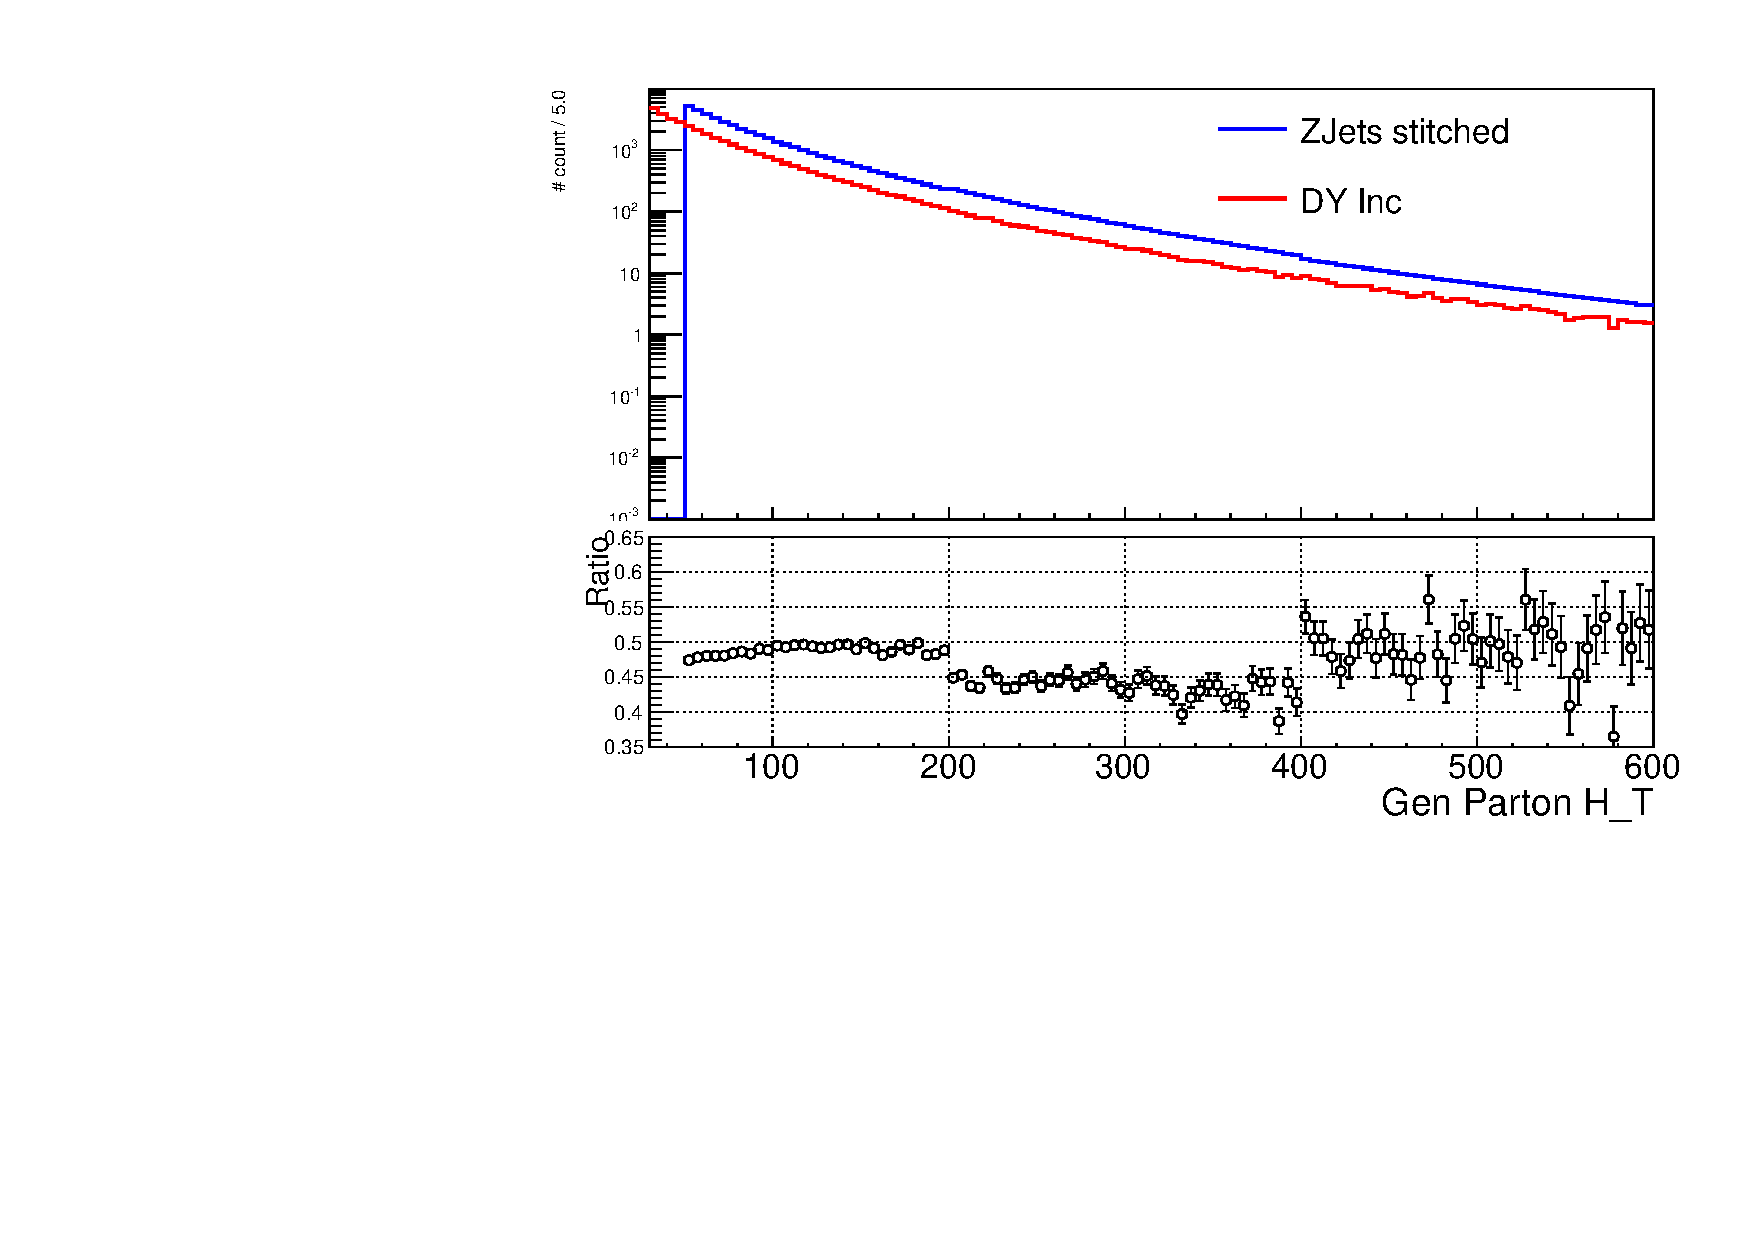
\includegraphics[width=\textwidth]{/Users/chrislucas/SUSY/thesis/Figs/xs_study/compar_genPartonHT_zmass_0_inc_inc_DYZJets_noCuts_sitv_log_HCPxS.pdf}
    \caption{No corrections.}
    \label{fig:xsec_study_before}
  \end{subfigure}             
  \begin{subfigure}[b]{0.45\textwidth}
    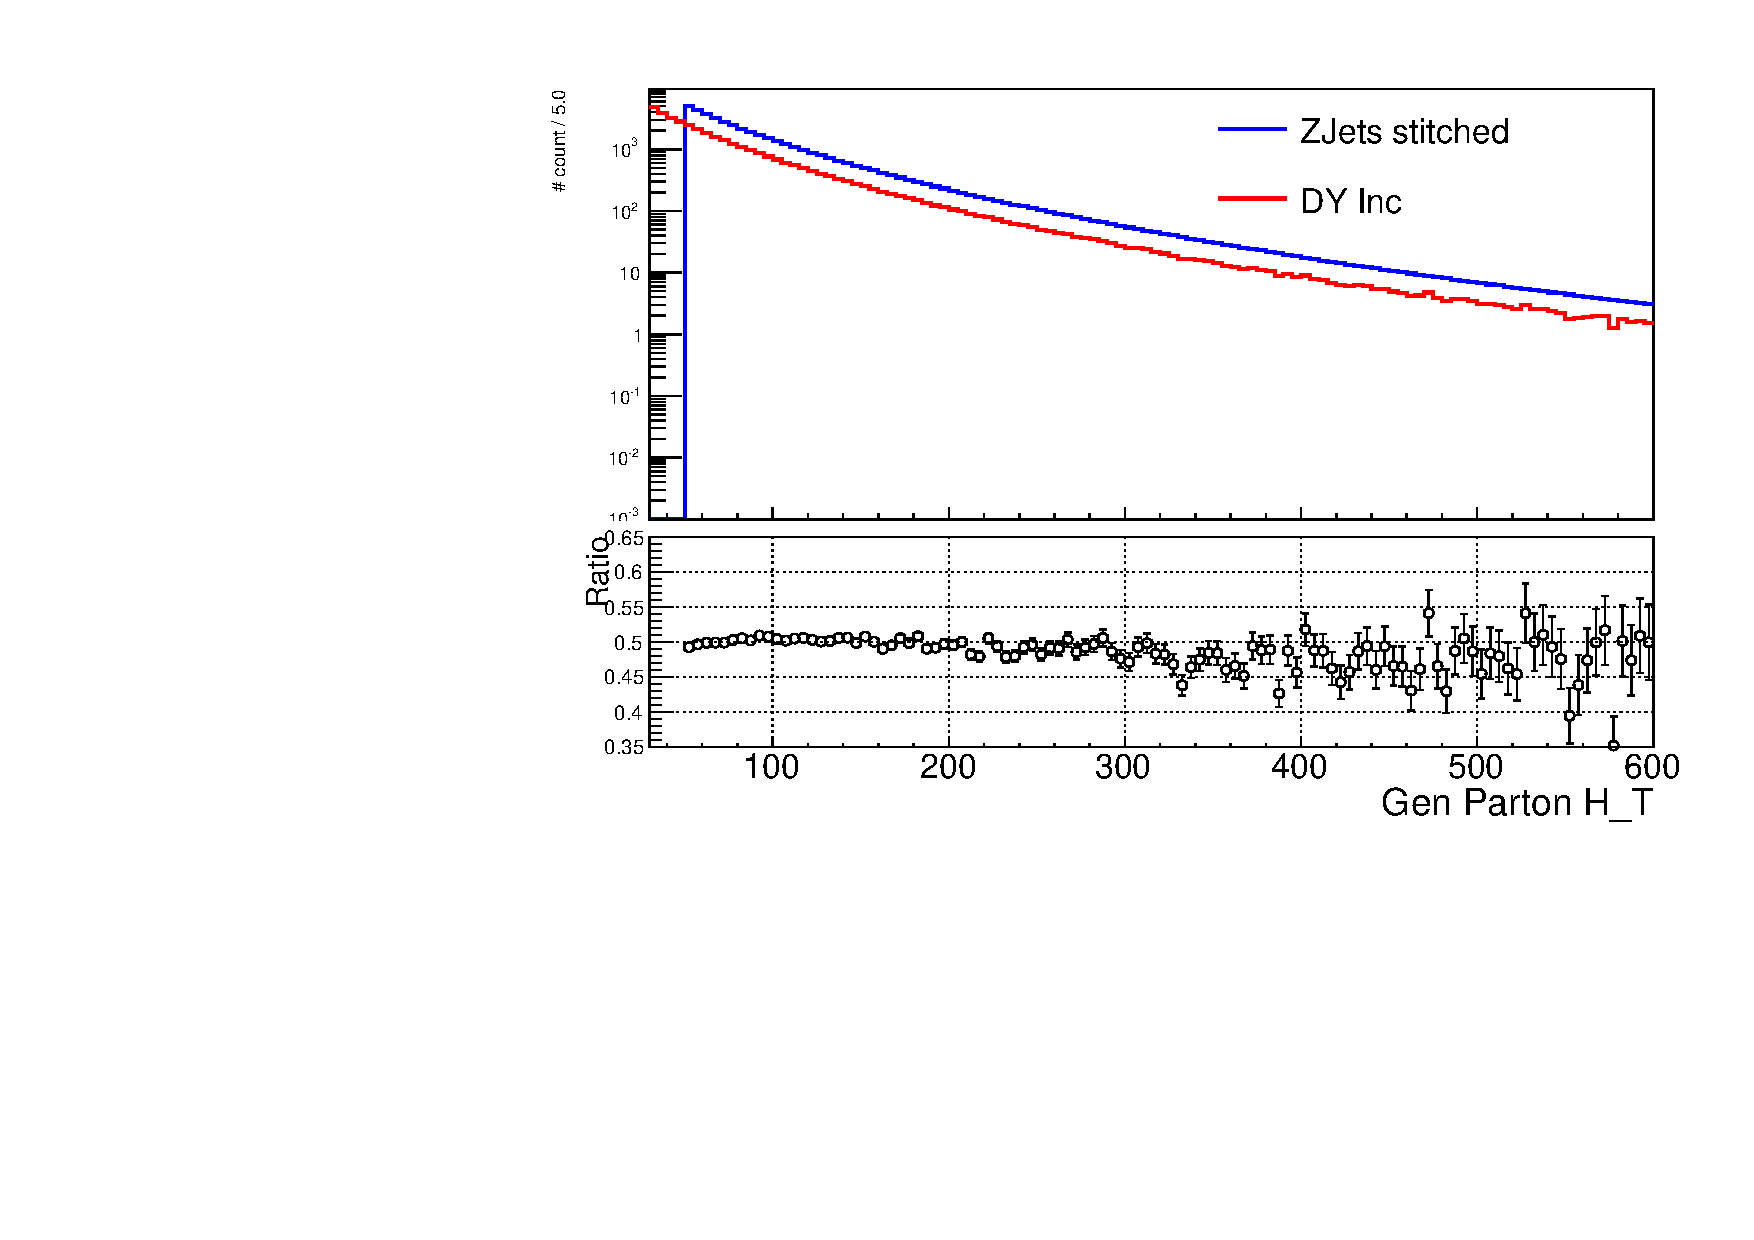
\includegraphics[width=\textwidth]{/Users/chrislucas/SUSY/thesis/Figs/xs_study/compar_genPartonHT_zmass_0_inc_inc_DYZJets_noCuts_sitv_log.pdf}
    \caption{With corrections.}
    \label{fig:xsec_study_after}
  \end{subfigure}             
  \caption{Generator-level \HTpart distributions from the
    inclusive DY + jets and the \HTpart-binned \zj
    samples.}
  \label{fig:xsec_study}
\end{figure}

Two of the binned samples have corresponding inclusive samples to allow for 
this comparison to be made, namely \wj and \dyj. For these two cases, the 
derivation of corrections for each \HTpart binned sample is simple. However, for 
\zj and \gj, no such inclusive samples exist. These binned samples are 
compared against the inclusive \dyj sample, where the overall normalisation is 
set according to the relative branching fraction of \zinv and GAMMA to
$Z \to \ell\ell$, set as 0.505 and VALUE, respectively. An example ratio plot is
shown in figure~\ref{fig:xsec_study_after}, where a constant ratio between the 
samples is found.

